 \section{Choix}
 Dans cette partie, nous allons présenter quelques uns des choix que
 nous avons faits concernant notre programme.

  \subsection{Langage}
  Nous avions le choix de faire ce projet en \emph{C} ou en
  \emph{C++}. Nous avons choisi \emph{C++} pour la simple raison que des
  structures de données intéressantes (notamment \emph{vector}) sont
  déjà présentes dans ce langage alors qu'elles ne le sont pas dans le
  langage \emph{C}.
  
  \subsection{Structure de données}
  Dans ce projet, nous avions à faire le choix d'une structure de
  données pour représenter les graphes. Nous avons suivi les conseils en
  décidant d'utiliser des listes d'adjacence.

  Plusieurs raisons nous ont poussés à utiliser les listes d'adjacence
  plutôt que d'autres structures\footnote{Il n'y a ici, pas de bon choix
  à proprement parler, le mieux serait de faire au cas par cas (nous en
  parlerons dans le bilan du rapport).} :
  \begin{enumerate}
   \item La liste d'adjacence est une des structures qui prend le moins
	 de place en mémoire car elle ne stocke que les sommets voisins
	 (contrairement à une matrice d'adjacence par exemple).
   \item La liste d'adjacence est très efficace lorsqu'on a à
	 considérer la liste des voisins des sommets (c'est son essence
	 même), ce qui est le cas pour nos réductions.
   \item La liste d'adjacence est évidemment plus efficace que n'importe
	 quelle structure d'incidence lorsqu'il s'agit de considérer les
	 sommets plutôt que les arêtes.
  \end{enumerate}

    \subsection{Dépendances et Relations}
  Le programme est simple d'utilisation puisqu'il suffit de le lancer
  avec un fichier d'entrée de type graphe issu du programme
  \emph{gengraph} de
  \emph{C. Gavoille}\footnote{\url{http://dept-info.labri.fr/~gavoille/gengraph.c}}
  ainsi qu'avec le numéro du problème et éventuellement des paramètres
  propres au problème.\\
  Le programme se déroule de la manière suivante :
  \begin{enumerate}
   \item Le fichier de graphe est lu à partir du fichier de graphe
	 fourni. 
   \item Selon le problème sélectionné, on lance la réduction
	 correspondante. 
   \item Une formulation en clauses de type \emph{CNF} est créée et
	 envoyée au \emph{SATSolver} \emph{Minisat}. 
   \item \emph{Minisat} crée une solution (si cela est possible).
   \item La solution fournie est analysée afin de pouvoir être
	 traitée. De cette manière, nous connaissons la solution au
	 problème voulu sur le graphe passé en paramètre. 
  \end{enumerate}
  
  En décrivant l'exécution du programme de cette façon, il est aisé de
  voir apparaître les relations entre les modules de notre programme.

  La fonction principale \emph{main}, contenue dans \emph{Solve.cpp},
  joue le rôle du tri des arguments et de construction du
  graphe. Ensuite, est appelée la réduction voulue, contenue dans les
  fichiers portant le nom d'un problème (ou leur abréviation). Une fois
  la réduction effectuée par ce fichier, celui-ci appelle un ``parser''
  pour \emph{Minisat} (dans \emph{MinisatBuilder.cpp}) qui gère le fait
  d'écrire un fichier d'entrée à \emph{Minisat}, de lancer le
  \emph{SAT-Solver} et d'analyser sa sortie. Une fois la sortie
  analysée, une assignation des variables est donnée. Celle-ci nous
  permet alors de fournir l'ensemble des arêtes ou sommets nécessaire
  définissant une solution du problème donné sur le graphe donné.\\

  Voici un graphe représentant simplement les relations entre les
  différentes parties du programme (fig.\ref{grapheExec} page
  \pageref{grapheExec}).
  \begin{figure}[!ht]
   \begin{center}
    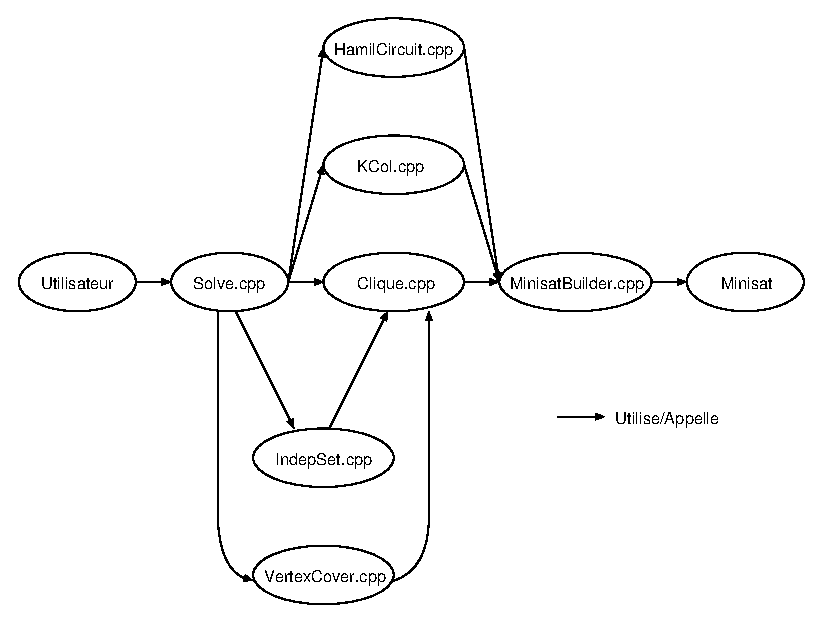
\includegraphics{images/grapheExec.eps}
    \caption{Relations entre les différentes parties du
    programme\label{grapheExec}}
   \end{center}
  \end{figure}

  \subsection{Extension des fichiers}
  Étant donné que nous générons des fichiers avec notre programme, nous
  avons choisi des extensions différentes selon le but du fichier.

  En effet nous avons introduit trois extensions différentes :
  \begin{enumerate}
   \item \emph{graph.gin} $\leadsto$ Fichier graphe de type
	 \emph{gengraph} passé en paramètre par l'utilisateur au
	 programme.
   \item \emph{graph.sat} $\leadsto$ Fichier qui contient la formule de
	 type \emph{CNF\footnote{\emph{Conjunctive Normal Form}}}
	 générée par notre programme à partir du choix du problème et du
	 graphe.
   \item \emph{graph.sol} $\leadsto$ Fichier qui contient la solution
	 retournée par \emph{Minisat}.
  \end{enumerate}

  Nous avons fait le choix de laisser ces fichiers sur le disque après
  exécution du programme, dans le cas où l'utilisateur souhaiterait y
  jeter un \oe{}il\footnote{Les utilisateurs que nous sommes ont
  beaucoup apprécié cette possibilité.}.
